A three-step selection process was carried out to identify the study area. First, the initial boundary of the study area was established as the union of all areas encompassed by or intersecting the catchment area of the sewer network serviced by the main wastewater treatment plant (WWTP) in Bologna. Next, any areas enclosed by the initially selected regions were included. Finally, areas primarily associated with other treatment facilities were excluded from the selection. This process resulted in a study area encompassing nearly all the census sections of Bologna, and a portion of the census sections of the neighbouring municipalities (Figure \ref{fig:area}). \\

\begin{figure}[b!]
\centering
\caption{Map of the study area (orange), wastewater treatment plant (red triangle), sewer network (blue), catchment area (light blue).}
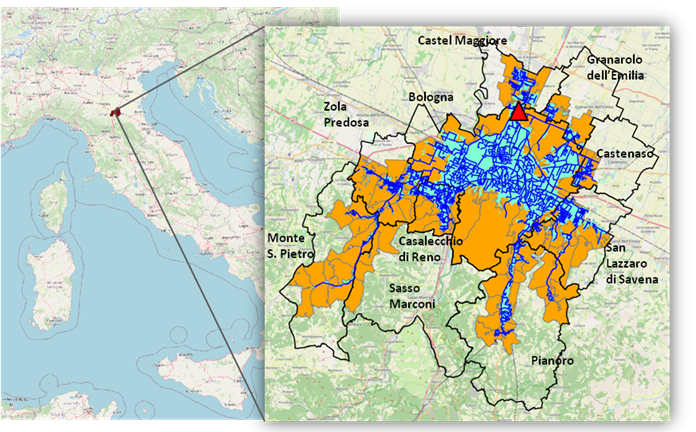
\includegraphics[width=0.95\textwidth]{area_paper.png}
\label{fig:area}
\end{figure}

To assess the performance of models described by (Contreras-Espinoza et al., 2023), data on newly reported COVID-19 cases provided by the Local Health Authority of Bologna were used. Specifically, employed data spans from October 13, 2021, to April 4, 2023, covering daily new cases within the WWTP service area. For each confirmed COVID-19 case, further detailed information is also available, including the census area where isolation took place, presence and onset date of symptoms, date of the swab test, diagnosis date, hospital admission and discharge dates, outcome (whether recovery or death), outcome date, and, if applicable, cause of death if applicable. \\

The time series data used in this project is available in the file \texttt{dati.xlsx}.